% Options for packages loaded elsewhere
\PassOptionsToPackage{unicode}{hyperref}
\PassOptionsToPackage{hyphens}{url}
%
\documentclass[
]{book}
\usepackage{lmodern}
\usepackage{amssymb,amsmath}
\usepackage{ifxetex,ifluatex}
\ifnum 0\ifxetex 1\fi\ifluatex 1\fi=0 % if pdftex
  \usepackage[T1]{fontenc}
  \usepackage[utf8]{inputenc}
  \usepackage{textcomp} % provide euro and other symbols
\else % if luatex or xetex
  \usepackage{unicode-math}
  \defaultfontfeatures{Scale=MatchLowercase}
  \defaultfontfeatures[\rmfamily]{Ligatures=TeX,Scale=1}
\fi
% Use upquote if available, for straight quotes in verbatim environments
\IfFileExists{upquote.sty}{\usepackage{upquote}}{}
\IfFileExists{microtype.sty}{% use microtype if available
  \usepackage[]{microtype}
  \UseMicrotypeSet[protrusion]{basicmath} % disable protrusion for tt fonts
}{}
\makeatletter
\@ifundefined{KOMAClassName}{% if non-KOMA class
  \IfFileExists{parskip.sty}{%
    \usepackage{parskip}
  }{% else
    \setlength{\parindent}{0pt}
    \setlength{\parskip}{6pt plus 2pt minus 1pt}}
}{% if KOMA class
  \KOMAoptions{parskip=half}}
\makeatother
\usepackage{xcolor}
\IfFileExists{xurl.sty}{\usepackage{xurl}}{} % add URL line breaks if available
\IfFileExists{bookmark.sty}{\usepackage{bookmark}}{\usepackage{hyperref}}
\hypersetup{
  pdftitle={R aplicado a suinocultura},
  pdfauthor={Marcio Valk},
  hidelinks,
  pdfcreator={LaTeX via pandoc}}
\urlstyle{same} % disable monospaced font for URLs
\usepackage{color}
\usepackage{fancyvrb}
\newcommand{\VerbBar}{|}
\newcommand{\VERB}{\Verb[commandchars=\\\{\}]}
\DefineVerbatimEnvironment{Highlighting}{Verbatim}{commandchars=\\\{\}}
% Add ',fontsize=\small' for more characters per line
\usepackage{framed}
\definecolor{shadecolor}{RGB}{248,248,248}
\newenvironment{Shaded}{\begin{snugshade}}{\end{snugshade}}
\newcommand{\AlertTok}[1]{\textcolor[rgb]{0.94,0.16,0.16}{#1}}
\newcommand{\AnnotationTok}[1]{\textcolor[rgb]{0.56,0.35,0.01}{\textbf{\textit{#1}}}}
\newcommand{\AttributeTok}[1]{\textcolor[rgb]{0.77,0.63,0.00}{#1}}
\newcommand{\BaseNTok}[1]{\textcolor[rgb]{0.00,0.00,0.81}{#1}}
\newcommand{\BuiltInTok}[1]{#1}
\newcommand{\CharTok}[1]{\textcolor[rgb]{0.31,0.60,0.02}{#1}}
\newcommand{\CommentTok}[1]{\textcolor[rgb]{0.56,0.35,0.01}{\textit{#1}}}
\newcommand{\CommentVarTok}[1]{\textcolor[rgb]{0.56,0.35,0.01}{\textbf{\textit{#1}}}}
\newcommand{\ConstantTok}[1]{\textcolor[rgb]{0.00,0.00,0.00}{#1}}
\newcommand{\ControlFlowTok}[1]{\textcolor[rgb]{0.13,0.29,0.53}{\textbf{#1}}}
\newcommand{\DataTypeTok}[1]{\textcolor[rgb]{0.13,0.29,0.53}{#1}}
\newcommand{\DecValTok}[1]{\textcolor[rgb]{0.00,0.00,0.81}{#1}}
\newcommand{\DocumentationTok}[1]{\textcolor[rgb]{0.56,0.35,0.01}{\textbf{\textit{#1}}}}
\newcommand{\ErrorTok}[1]{\textcolor[rgb]{0.64,0.00,0.00}{\textbf{#1}}}
\newcommand{\ExtensionTok}[1]{#1}
\newcommand{\FloatTok}[1]{\textcolor[rgb]{0.00,0.00,0.81}{#1}}
\newcommand{\FunctionTok}[1]{\textcolor[rgb]{0.00,0.00,0.00}{#1}}
\newcommand{\ImportTok}[1]{#1}
\newcommand{\InformationTok}[1]{\textcolor[rgb]{0.56,0.35,0.01}{\textbf{\textit{#1}}}}
\newcommand{\KeywordTok}[1]{\textcolor[rgb]{0.13,0.29,0.53}{\textbf{#1}}}
\newcommand{\NormalTok}[1]{#1}
\newcommand{\OperatorTok}[1]{\textcolor[rgb]{0.81,0.36,0.00}{\textbf{#1}}}
\newcommand{\OtherTok}[1]{\textcolor[rgb]{0.56,0.35,0.01}{#1}}
\newcommand{\PreprocessorTok}[1]{\textcolor[rgb]{0.56,0.35,0.01}{\textit{#1}}}
\newcommand{\RegionMarkerTok}[1]{#1}
\newcommand{\SpecialCharTok}[1]{\textcolor[rgb]{0.00,0.00,0.00}{#1}}
\newcommand{\SpecialStringTok}[1]{\textcolor[rgb]{0.31,0.60,0.02}{#1}}
\newcommand{\StringTok}[1]{\textcolor[rgb]{0.31,0.60,0.02}{#1}}
\newcommand{\VariableTok}[1]{\textcolor[rgb]{0.00,0.00,0.00}{#1}}
\newcommand{\VerbatimStringTok}[1]{\textcolor[rgb]{0.31,0.60,0.02}{#1}}
\newcommand{\WarningTok}[1]{\textcolor[rgb]{0.56,0.35,0.01}{\textbf{\textit{#1}}}}
\usepackage{longtable,booktabs}
% Correct order of tables after \paragraph or \subparagraph
\usepackage{etoolbox}
\makeatletter
\patchcmd\longtable{\par}{\if@noskipsec\mbox{}\fi\par}{}{}
\makeatother
% Allow footnotes in longtable head/foot
\IfFileExists{footnotehyper.sty}{\usepackage{footnotehyper}}{\usepackage{footnote}}
\makesavenoteenv{longtable}
\usepackage{graphicx,grffile}
\makeatletter
\def\maxwidth{\ifdim\Gin@nat@width>\linewidth\linewidth\else\Gin@nat@width\fi}
\def\maxheight{\ifdim\Gin@nat@height>\textheight\textheight\else\Gin@nat@height\fi}
\makeatother
% Scale images if necessary, so that they will not overflow the page
% margins by default, and it is still possible to overwrite the defaults
% using explicit options in \includegraphics[width, height, ...]{}
\setkeys{Gin}{width=\maxwidth,height=\maxheight,keepaspectratio}
% Set default figure placement to htbp
\makeatletter
\def\fps@figure{htbp}
\makeatother
\setlength{\emergencystretch}{3em} % prevent overfull lines
\providecommand{\tightlist}{%
  \setlength{\itemsep}{0pt}\setlength{\parskip}{0pt}}
\setcounter{secnumdepth}{5}
\usepackage{booktabs}
\usepackage{amsthm}
\usepackage{bbm}
\usepackage{url}

\newcommand{\Prob}[1]{
\mathbbm{P} \left( #1 \right)
}
\newcommand{\R}{\mathbb{R}}
\newcommand{\E}{\mathbb{E}}
\DeclareMathOperator{\cov}{cov}
\DeclareMathOperator{\cor}{cor}
\DeclareMathOperator{\var}{var}
\makeatletter
\def\thm@space@setup{%
  \thm@preskip=8pt plus 2pt minus 4pt
  \thm@postskip=\thm@preskip
}
\makeatother
\usepackage[]{natbib}
\bibliographystyle{apalike}

\title{R aplicado a suinocultura}
\author{Marcio Valk}
\date{2020-07-09}

\begin{document}
\frontmatter
\maketitle

{
\setcounter{tocdepth}{1}
\tableofcontents
}
\mainmatter
\hypertarget{objetivo}{%
\chapter*{Objetivo}\label{objetivo}}
\addcontentsline{toc}{chapter}{Objetivo}

O R tem se caracterizado por ser uma ferramenta completa para quem trabalha com pesquisa, seja aplicada ou teórica. As diversas áreas do conhecimento acabam convergindo para o R, por se tratar de uma linguagem moderna, dinâmica, colaborativa e integradora.

A pesquisa e o desenvolvimento tecnógico na área da suinocultura geram um volume considerável de informações que necessitam ser analisadas. O R é uma ferramenta que permite, ler, integrar e tratar grandes bancos de dados, é bem desenvolvido na área de visualização de dados e possui uma diverside de métodos estatísticos implementados. Além disso, ferramentas para gerar relatórios, apresentações e até mesmo a criação de aplicativos que possibilitam a interação do usuário final, tornam o R uma ferramenta completa.

\hypertarget{sobre-a-academia}{%
\section*{Sobre a Academia}\label{sobre-a-academia}}
\addcontentsline{toc}{section}{Sobre a Academia}

\begin{quote}
\emph{A Academia Suína foi fundada em 2018 para revolucionar a disseminação da educação na Suinocultura Brasileira. Contamos os maiores professores da Suinocultura Internacional, representando mais de 28 universidades, e com um foco prático e de alto impacto ao nível de granja}. \citep{academiasuina}
\end{quote}

\hypertarget{sobre-o-autor}{%
\section*{Sobre o autor}\label{sobre-o-autor}}
\addcontentsline{toc}{section}{Sobre o autor}

Meu nome é Marcio, sou professor do Departamento de Estatística da UFRGS e sou um grande fã do R. Encarei esse desafio pois gosto de pensar que outras áreas, além da Estatística, possam usufruir das fantásticas ferramentas que essa linguagem oferece. Além disso, contribuindo para o desenvolvimento tecnológio da área da suinucultura , estaremos contribuindo para o desenvolvimento do país.

\hypertarget{tuto}{%
\chapter{Tutorial básico R e RStudio}\label{tuto}}

\hypertarget{apresentauxe7uxe3o-da-linguagem-r}{%
\section{Apresentação da linguagem R}\label{apresentauxe7uxe3o-da-linguagem-r}}

R é uma linguagem de programação caracterizada como Software Livre sob os termos da \emph{General Public License (GNU)} da \emph{Free Software Foundation} no formato \emph{open source}. É voltada a manipulação, análise e vizualização de dados e tem como característica o aspecto colaborativo, sendo que as ferramentas desenvolvidas são compartilhadas online pelos desenvolvedores, podendo ter acesso a elas qualquer pessoa, sem restrições. Uma breve história do R pode ser encontrada no \href{https://pt.wikipedia.org/wiki/R_(linguagem_de_programa\%C3\%A7\%C3\%A3o)}{wikipedia}.

\hypertarget{instalando-o-r}{%
\section{Instalando o R}\label{instalando-o-r}}

Para instalar no computador, O R deve ser baixado do \href{https://cran.r-project.org/}{CRAN}.

\begin{figure}
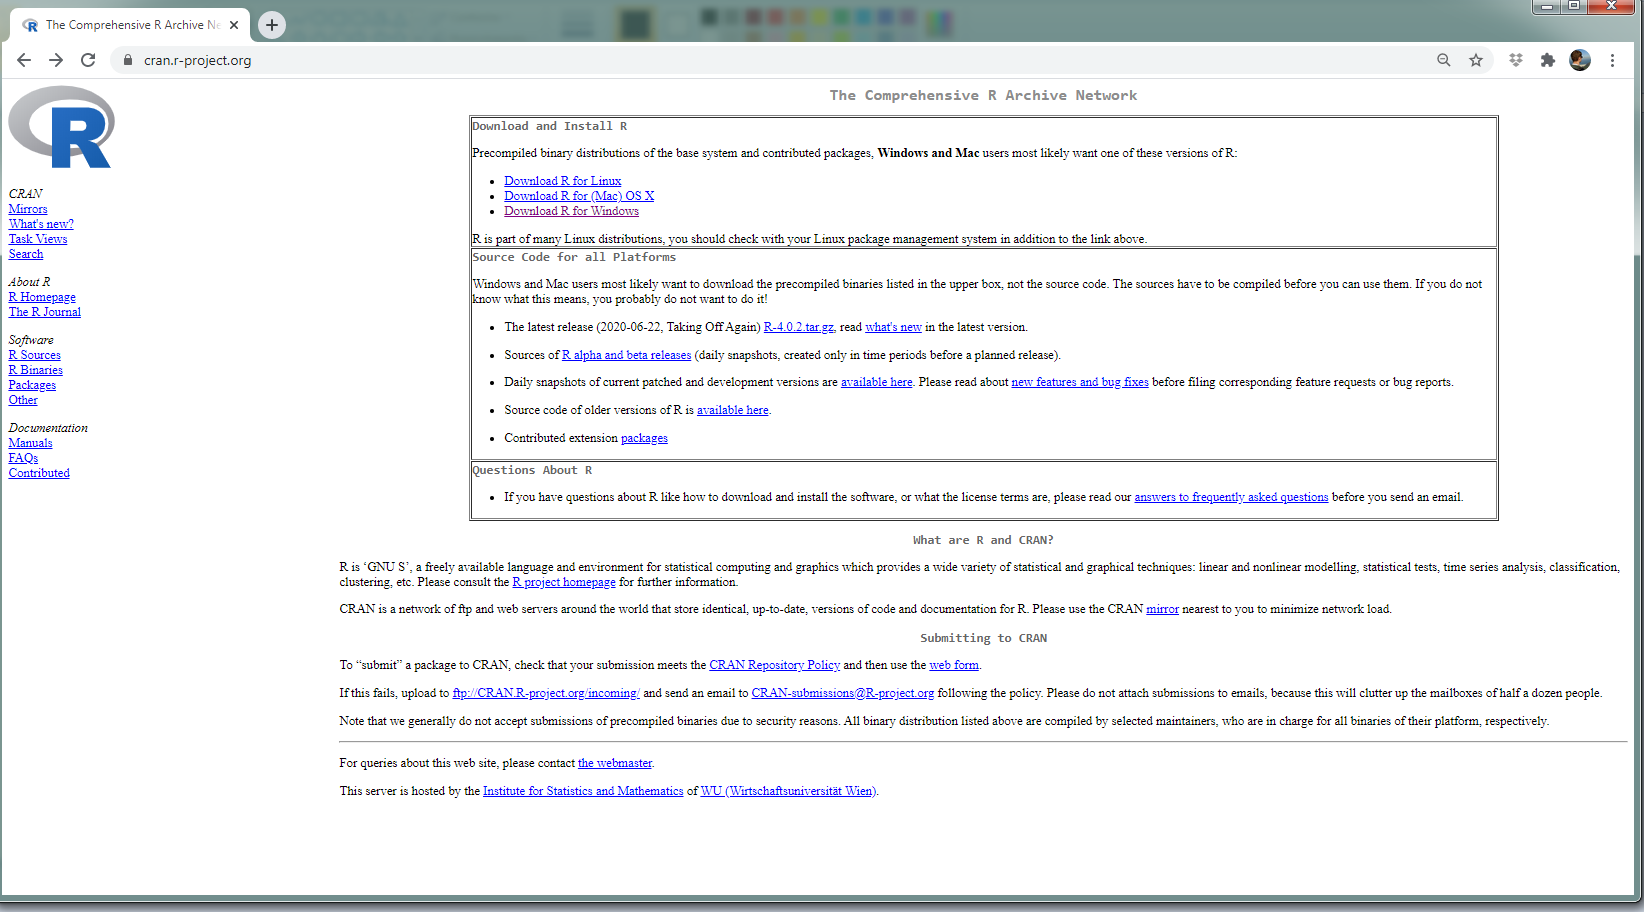
\includegraphics[width=0.9\linewidth]{Figuras/CRAN} \caption{Comprehensive R archive network (CRAN)}\label{fig:cran}
\end{figure}

Se o sistema operacional for Linux, uma versão \emph{base} do R ja vem instalada. No cado de outros sistemas operacionais, como o Windows, é necessário instalar o R \href{https://cran.r-project.org/bin/windows/base/}{base}.

\hypertarget{instalando-o-rstudio}{%
\section{Instalando o RStudio}\label{instalando-o-rstudio}}

Como quase toda linguagem \emph{Open Source} a utilização se dá por meio de linhas de comando. Para tornar a linguagem mais amigável aos usuários, várias IDEs (\emph{integrated development environment}) são utilizadas. No caso do R, a mais desenvolvida e utilizada é o \href{https://rstudio.com/products/rstudio/}{RStudio}.

Uma versão \emph{Free} do RStudio para o seu desktop pode ser baixado de \url{https://rstudio.com/products/rstudio/download/}.

Depois de instalar o R, o RStudio já estará integrado ao R e terá uma interface intuitiva e amigável ao usuário.

\begin{quote}
Ainda assim, é importante ressaltar que na linguagem R não encontraremos \emph{botões} para realizar as análises.
\end{quote}

\begin{figure}
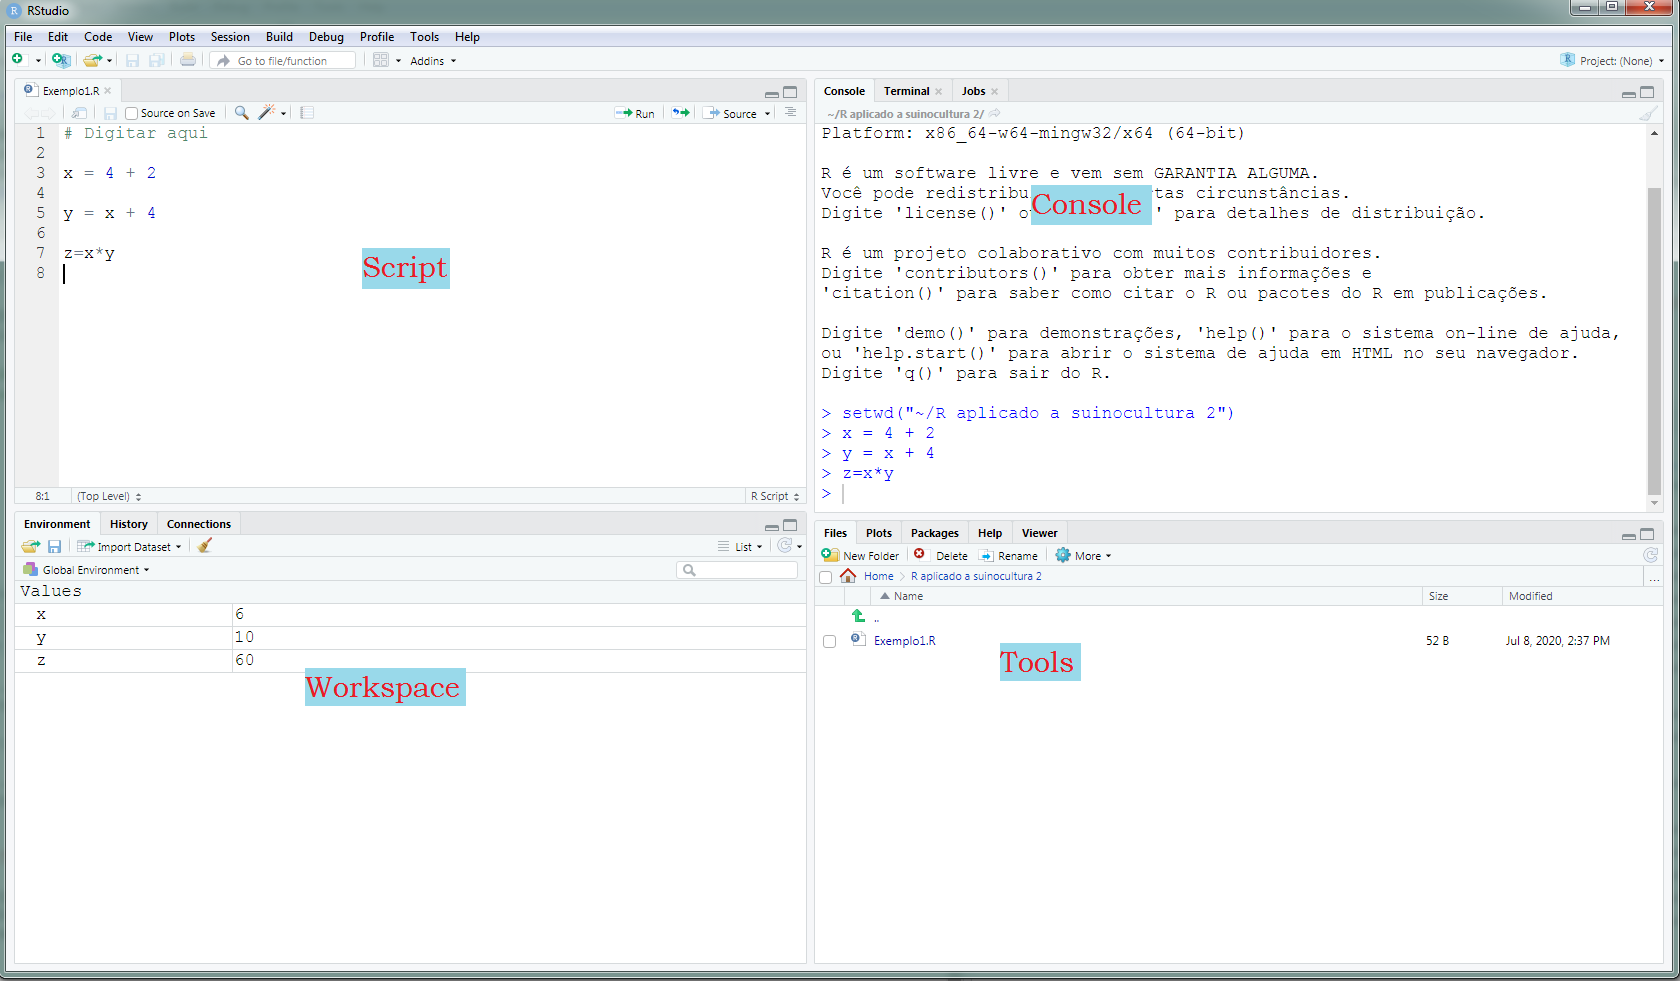
\includegraphics[width=0.9\linewidth]{Figuras/RStudio} \caption{Interface do RStudio}\label{fig:rstudio}
\end{figure}

\hypertarget{diretuxf3rio-de-trabalho}{%
\section{Diretório de trabalho}\label{diretuxf3rio-de-trabalho}}

Um ação importante que deve ser realizada pelo usuário é \emph{setar o diretório} de trabalho. Para isso existem diferentes formas. Uma delas é usando a função \emph{setwd()} .

\begin{Shaded}
\begin{Highlighting}[]
\KeywordTok{setwd}\NormalTok{(}\StringTok{"~/R aplicado a suinocultura 2"}\NormalTok{)}
\end{Highlighting}
\end{Shaded}

Outra opção é através do \emph{Go to directory} que está disponível no Workspace do RStudio, conforme figura \ref{fig:rstudio2}. Nessa opção o usuário escolhe o diretório de trabalho e depois usando a opção \emph{set as working directory} esse diretório será ``\emph{settado}'' como diretório de trabalho.

\begin{quote}
Todas os arquivos gerados, como figuras serão salvos nesse diretório. Para abrir um conjunto de dados, por exemplo, será muito mais simples se este também estiver salvo no mesmo diretório ou um subdiretório. Além disso, toda vez que o RStudio for reinicializado, esse procedimento terá que ser refeito.
\end{quote}

\begin{figure}
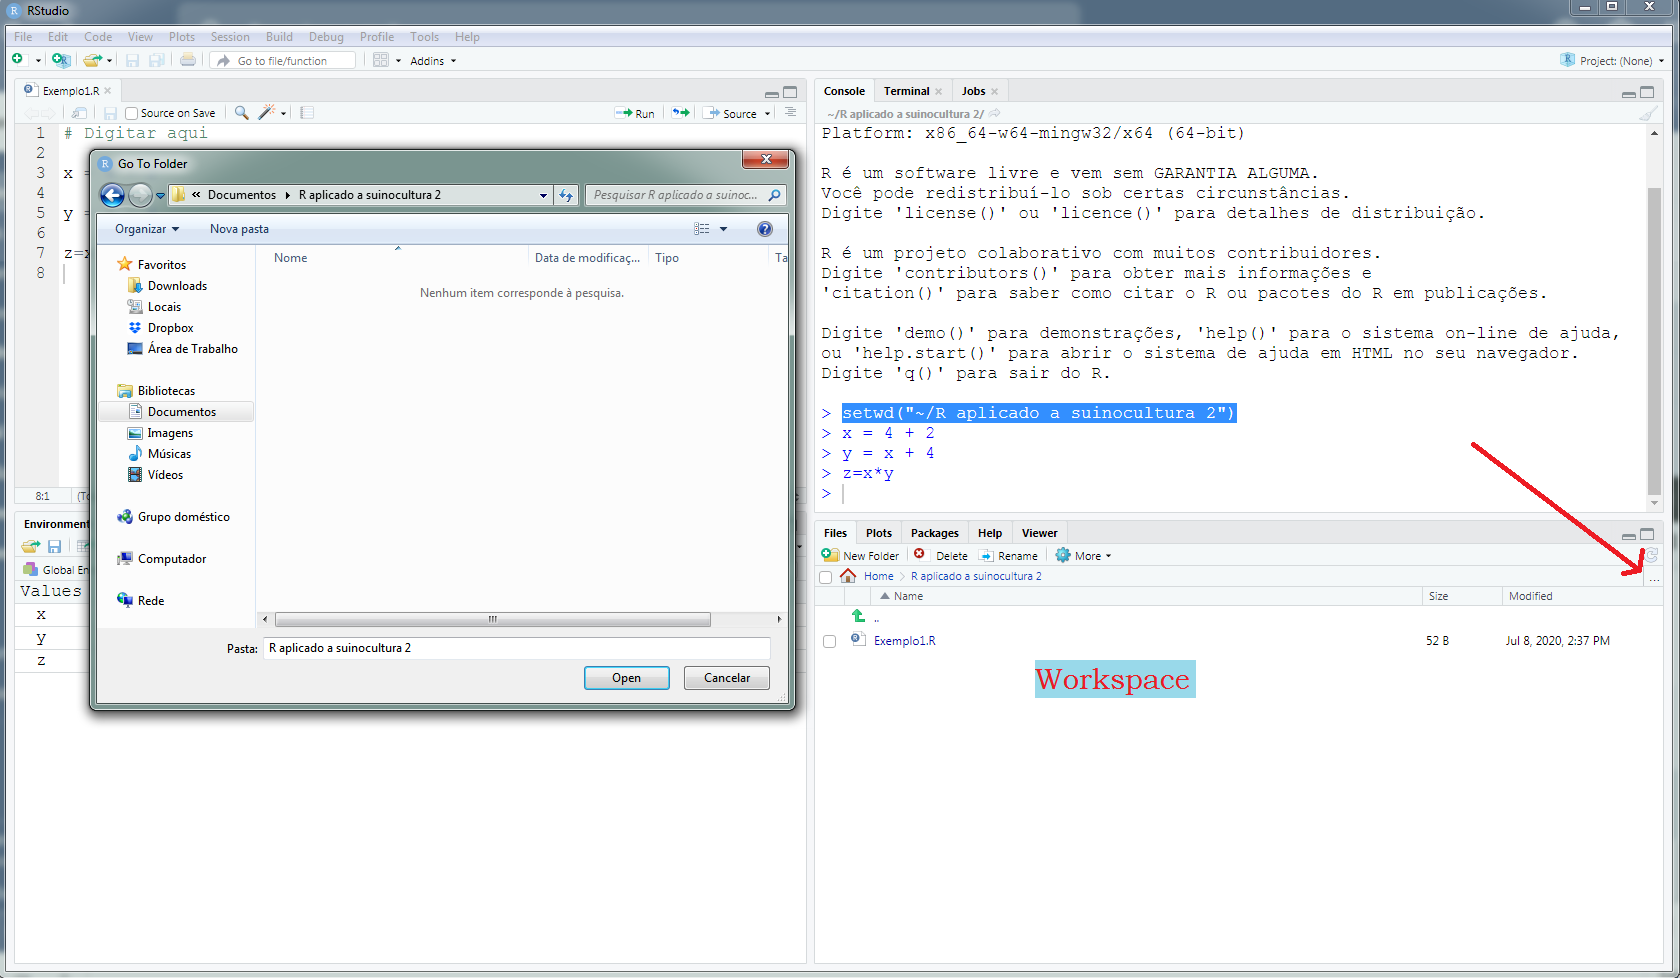
\includegraphics[width=0.46\linewidth]{Figuras/RStudio2} 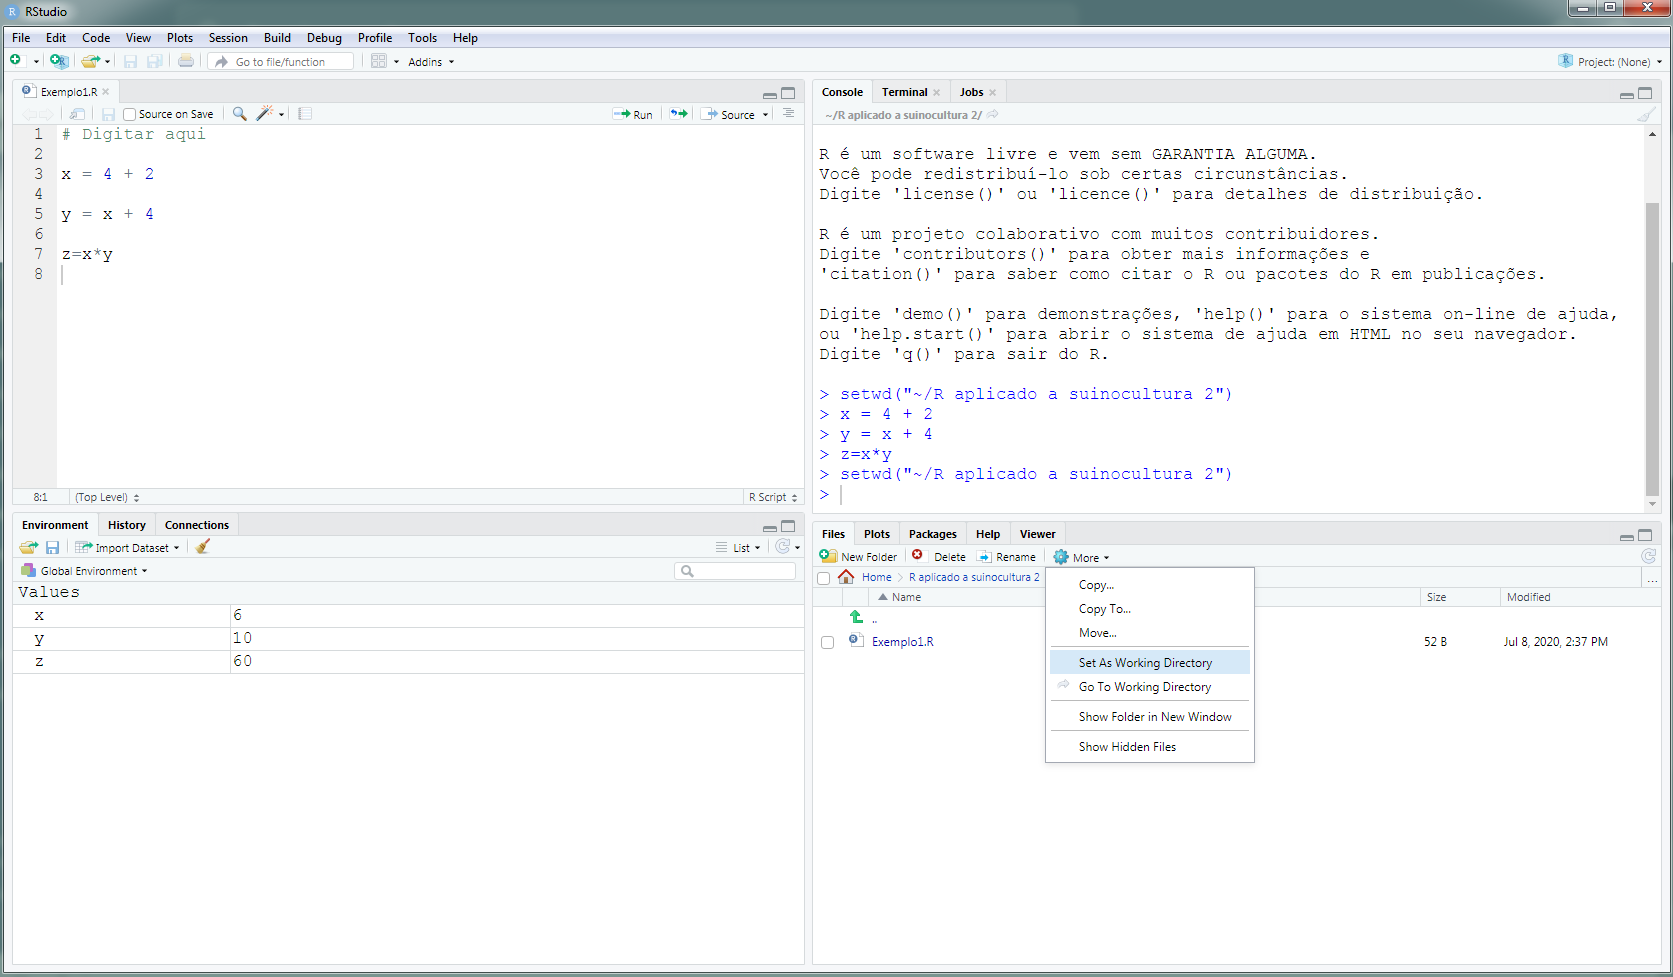
\includegraphics[width=0.46\linewidth]{Figuras/RStudio3} \caption{Diretório de trabalho}\label{fig:rstudio2}
\end{figure}

\hypertarget{rstudio-cloud}{%
\section{RStudio Cloud}\label{rstudio-cloud}}

Outra forma simples e prática para usar o R e o RStudio é usar o \href{https://rstudio.cloud/}{RStudio Cloud}.

\begin{quote}
\emph{THE MISSION
We created RStudio Cloud to make it easy for professionals, hobbyists, trainers, teachers and students to do, share, teach and learn data science}. \citep{rstudiocloud}
\end{quote}

\begin{figure}

\includegraphics[width=0.9\linewidth]{Figuras/RStudioCloud} \caption{Rstudio Cloud}\label{fig:rstudiocloud}
\end{figure}

Na núvem é possível usar o RStudio utilizando um login através da conta google, ou criar gratuitamente uma conta. Uma vez logado, escolhendo a opção \emph{project} o usuário terá uma versão do RStudio perfeitamente funcional, que pode ser utilizada até no smartphone. Obviamente, é necessário ter conexão com a internet para que a ferramenta possa ser utilizada.

\begin{figure}
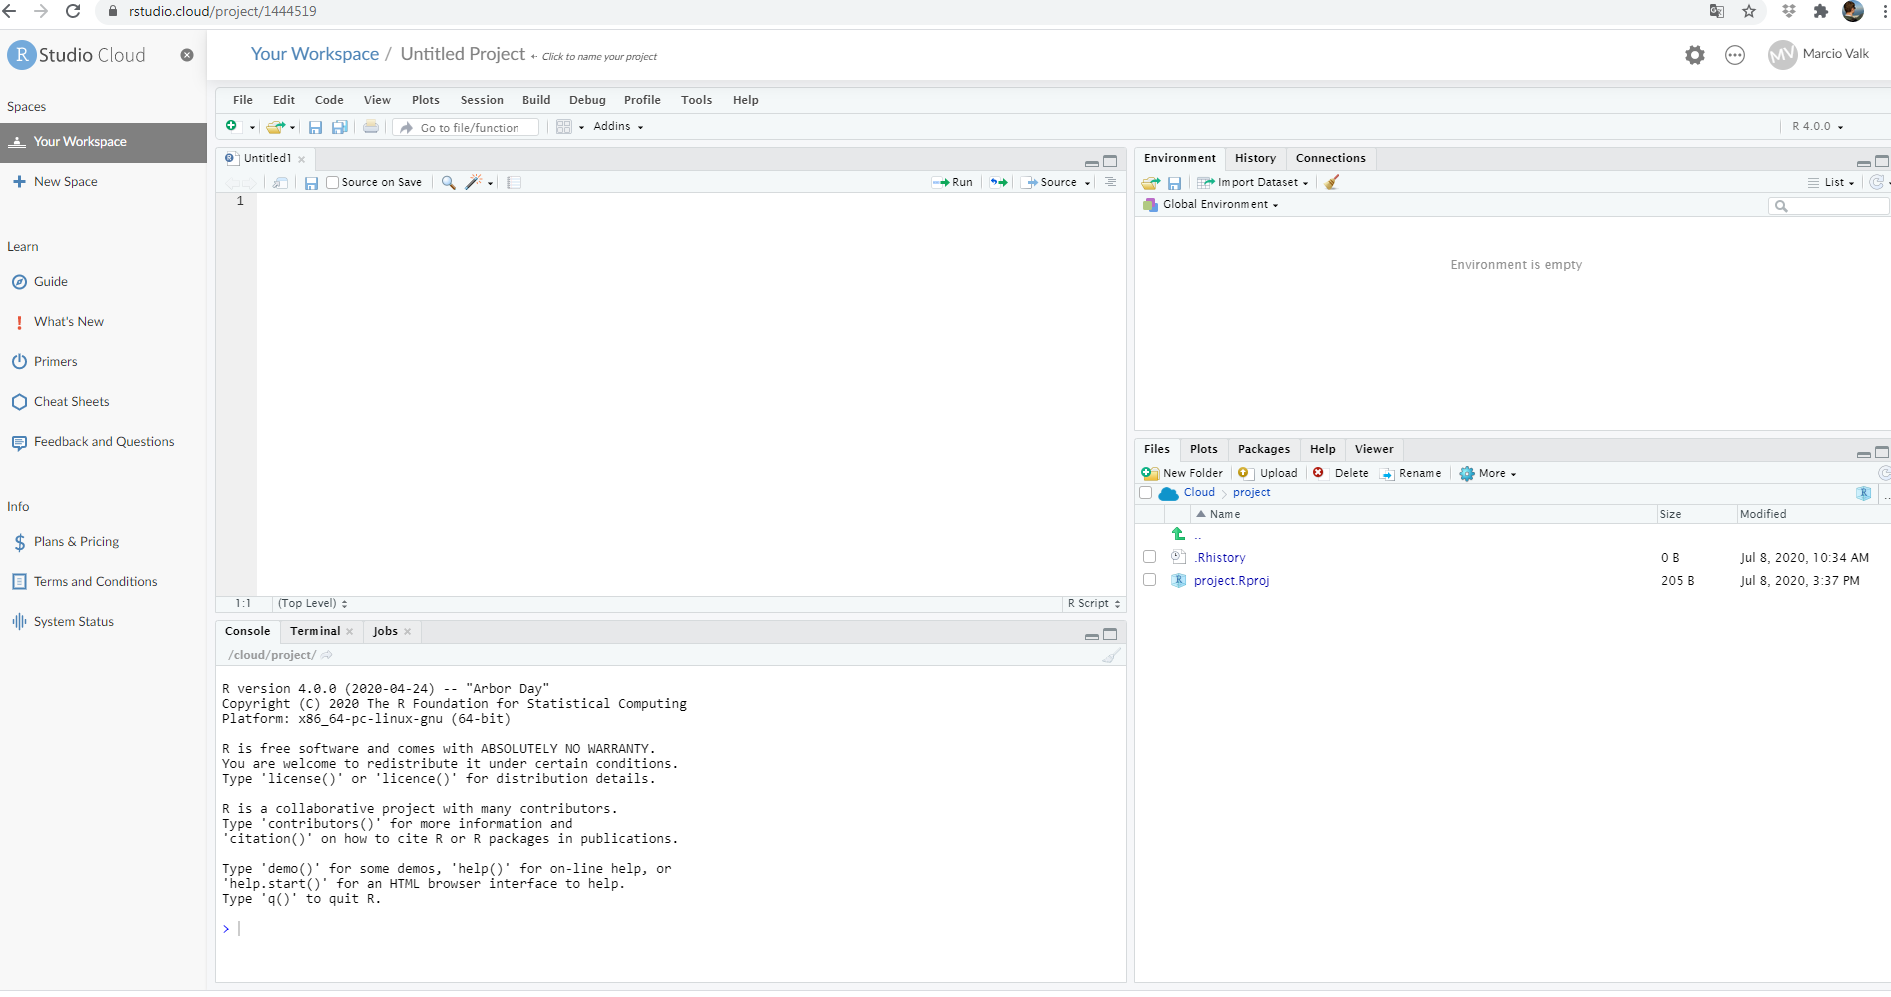
\includegraphics[width=0.9\linewidth]{Figuras/RStudioCloud2} \caption{Rstudio Cloud}\label{fig:rstudiocloud2}
\end{figure}

\hypertarget{instalauxe7uxe3o-de-pacotes}{%
\section{Instalação de pacotes}\label{instalauxe7uxe3o-de-pacotes}}

Na versão \emph{base} do R, uma série de ferramentas, funções e métodos estatísticos são disponibilizados. Além disso, alguns pacotes também compõe a versão \emph{base} do R. Depois de instalado, o usuário pode verificar quais pacotes estão instalados acessando o ícone \emph{Packages} n

\hypertarget{funcionalidades-buxe1sicas}{%
\section{Funcionalidades básicas}\label{funcionalidades-buxe1sicas}}

\hypertarget{operauxe7uxf5es}{%
\subsection{Operações}\label{operauxe7uxf5es}}

\hypertarget{operadores-luxf3gicos}{%
\subsection{Operadores lógicos}\label{operadores-luxf3gicos}}

\hypertarget{variuxe1veis-no-r}{%
\section{Variáveis no R}\label{variuxe1veis-no-r}}

\hypertarget{operauxe7uxf5es-1}{%
\subsection{Operações}\label{operauxe7uxf5es-1}}

\hypertarget{vetores}{%
\section{Vetores}\label{vetores}}

\hypertarget{operauxe7uxf5es-com-vetores}{%
\subsection{Operações com vetores}\label{operauxe7uxf5es-com-vetores}}

\hypertarget{matrizes}{%
\section{Matrizes}\label{matrizes}}

\hypertarget{operauxe7uxf5es-com-matrizes}{%
\subsection{Operações com Matrizes}\label{operauxe7uxf5es-com-matrizes}}

\hypertarget{uso-do-for-loop}{%
\section{Uso do for (loop)}\label{uso-do-for-loop}}

\hypertarget{funuxe7uxf5es}{%
\section{Funções}\label{funuxe7uxf5es}}

\hypertarget{import}{%
\chapter{Importando dados}\label{import}}

\hypertarget{dados-de-diferentes-formatos}{%
\section{Dados de diferentes formatos}\label{dados-de-diferentes-formatos}}

\hypertarget{dados-no-formato-.txt}{%
\subsection{Dados no formato .txt}\label{dados-no-formato-.txt}}

\hypertarget{dados-no-formato-.csv}{%
\subsection{Dados no formato .csv}\label{dados-no-formato-.csv}}

\hypertarget{dados-no-formato-.xls-e-.xlsx}{%
\subsection{Dados no formato .xls e .xlsx}\label{dados-no-formato-.xls-e-.xlsx}}

\hypertarget{dados-do-sas-spss-e-stata}{%
\subsection{Dados do SAS, SPSS e STATA}\label{dados-do-sas-spss-e-stata}}

\hypertarget{dados-de-um-reposituxf3rio-web}{%
\subsection{Dados de um repositório web}\label{dados-de-um-reposituxf3rio-web}}

\hypertarget{anuxe1lise-exploratuxf3ria}{%
\section{Análise exploratória}\label{anuxe1lise-exploratuxf3ria}}

\hypertarget{dados-faltantes}{%
\subsection{Dados faltantes}\label{dados-faltantes}}

\hypertarget{anuxe1lise-exploratuxf3ria-1}{%
\section{Análise exploratória}\label{anuxe1lise-exploratuxf3ria-1}}

\hypertarget{medidas-de-tenduxeancia-central}{%
\subsection{Medidas de tendência central}\label{medidas-de-tenduxeancia-central}}

Média, mediana, variância

\hypertarget{plot-simples}{%
\subsection{Plot simples}\label{plot-simples}}

\hypertarget{box-plot-simples}{%
\subsection{Box plot simples}\label{box-plot-simples}}

\hypertarget{box-plot-multiplas-vuxe1riuxe1veis}{%
\subsection{Box plot multiplas váriáveis}\label{box-plot-multiplas-vuxe1riuxe1veis}}

\hypertarget{scater-plot}{%
\subsection{Scater plot}\label{scater-plot}}

\hypertarget{qqplot}{%
\subsection{QQplot}\label{qqplot}}

\hypertarget{anuxe1lise-estatuxedstica-de-dados---modelagem}{%
\section{Análise estatística de dados - Modelagem}\label{anuxe1lise-estatuxedstica-de-dados---modelagem}}

\hypertarget{regressuxe3o-linear-simples}{%
\subsection{Regressão linear simples}\label{regressuxe3o-linear-simples}}

\hypertarget{regressuxe3o-muxfaltipa}{%
\subsection{Regressão Múltipa}\label{regressuxe3o-muxfaltipa}}

\hypertarget{gruxe1ficos-de-resuxedduos}{%
\subsection{Gráficos de resíduos}\label{gruxe1ficos-de-resuxedduos}}

\hypertarget{studentized-residuals}{%
\subsubsection{studentized residuals}\label{studentized-residuals}}

\hypertarget{outliers}{%
\subsubsection{outliers}\label{outliers}}

\hypertarget{normalidade}{%
\subsubsection{normalidade}\label{normalidade}}

\hypertarget{anova-one-way}{%
\subsection{Anova one way}\label{anova-one-way}}

\hypertarget{visu}{%
\chapter{Visualização de dados com o R}\label{visu}}

\hypertarget{ggplot-anatomia-e-a-estrutura-data.frame}{%
\section{ggplot, anatomia e a estrutura data.frame}\label{ggplot-anatomia-e-a-estrutura-data.frame}}

\hypertarget{funuxe7uxf5es-geom-e-aes}{%
\section{Funções geom e aes}\label{funuxe7uxf5es-geom-e-aes}}

\hypertarget{segmentauxe7uxe3o-e-junuxe7uxe3o-de-gruxe1ficos-do-ggplot}{%
\section{Segmentação e junção de gráficos do ggplot}\label{segmentauxe7uxe3o-e-junuxe7uxe3o-de-gruxe1ficos-do-ggplot}}

\hypertarget{diferentes-tipos-de-gruxe1ficos}{%
\section{Diferentes tipos de gráficos}\label{diferentes-tipos-de-gruxe1ficos}}

\hypertarget{gruxe1fico-de-relacionamento}{%
\subsection{Gráfico de relacionamento}\label{gruxe1fico-de-relacionamento}}

\hypertarget{gruxe1ficos-de-barras}{%
\subsection{Gráficos de barras}\label{gruxe1ficos-de-barras}}

\hypertarget{gruxe1fico-de-suxe9ries-temporais}{%
\subsection{Gráfico de séries temporais}\label{gruxe1fico-de-suxe9ries-temporais}}

\hypertarget{mapas-de-calor}{%
\subsection{Mapas de calor}\label{mapas-de-calor}}

\hypertarget{box-plot}{%
\subsection{box plot}\label{box-plot}}

\hypertarget{ade}{%
\chapter{Análise de delineamento de experimentos}\label{ade}}

\hypertarget{delineamento-inteiramente-casualizados}{%
\section{Delineamento inteiramente casualizados}\label{delineamento-inteiramente-casualizados}}

\hypertarget{delineamento-em-blocos-ao-acaso}{%
\section{Delineamento em blocos ao acaso}\label{delineamento-em-blocos-ao-acaso}}

\hypertarget{fatorial}{%
\section{Fatorial}\label{fatorial}}

\hypertarget{parcela-subdividida}{%
\section{Parcela subdividida}\label{parcela-subdividida}}

\hypertarget{rmd}{%
\chapter{Relatórios e artigos científicos com o rmarkdown}\label{rmd}}

\hypertarget{relatuxf3rio-dinuxe2mico-com-o-rmarkdown}{%
\section{Relatório dinâmico com o Rmarkdown}\label{relatuxf3rio-dinuxe2mico-com-o-rmarkdown}}

\hypertarget{relatuxf3rios-em-word-pdf-ou-html}{%
\section{Relatórios em word, pdf ou html}\label{relatuxf3rios-em-word-pdf-ou-html}}

\hypertarget{apresentauxe7uxf5es-em-power-point}{%
\section{Apresentações em Power Point}\label{apresentauxe7uxf5es-em-power-point}}

\backmatter
  \bibliography{book.bib,packages.bib}

\end{document}
